\section{Исследуемые закономерности}

В состав экспериментальной установки входит нагретая до высокой (\( T \sim 1000\,\text{K} \)) температуры тонкая металлическая пластина с площадью поверхности \( S = 0{,}25\,\text{см}^2 \). Пластина относится к числу серых тел, поглощательная способность которой равна \( \alpha_T = 0{,}92 \). В процессе эксперимента измеряются мощность Джоуля–Ленца \( P = UI \), выделяемая в пластине, и переходящая в мощность теплового излучения пластины \( P_{\text{ти}} \). В условиях теплового равновесия:

\[
P_{\text{ти}} = \alpha \sigma T^4 = P = UI
\]

Для измерения температуры \( T \) пластины используется неконтактный термометр (оптический пирометр).

Через окуляр зрительной трубы пирометра наблюдатель видит (рис.~\ref{fig:brightness_combined}, а) светящуюся нить (основная часть пирометра) на фоне светящейся поверхности исследуемого тела. Увеличение силы тока в нити пирометра приводит к возрастанию её температуры и яркости свечения. При определённой яркости нить становится невидимой (рис.~\ref{fig:brightness_combined}, б) на фоне светящейся поверхности.

Если бы оба тела (нить и пластина) являлись бы абсолютно чёрными телами, то одинаковая яркость их свечения свидетельствовала бы о равенстве их температур. В экспериментальной же установке нить пирометра является эквивалентом абсолютно чёрного тела (АЧТ), а нагреваемая пластина относится к классу серых тел. Поэтому при одинаковой яркости чёрного и серого тел их температуры \( T_n \) и \( T \) будут различны.

\begin{figure}[htb]
    \centering
    \begin{minipage}{0.45\textwidth}
        \centering
        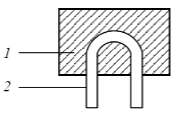
\includegraphics[width=0.8\textwidth]{images/fig_brightness_a.png}\\
        \small а
    \end{minipage}
    \hfill
    \begin{minipage}{0.45\textwidth}
        \centering
        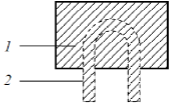
\includegraphics[width=0.8\textwidth]{images/fig_brightness_b.png}\\
        \small б
    \end{minipage}
    \caption{Видимое изображение нагретой нити 2 на фоне светящейся поверхности исследуемого тела при разной (а) и одинаковой (б) светимости тел}
    \label{fig:brightness_combined}
\end{figure}

Оптический пирометр проградуирован по температуре АЧТ, и в опыте мы измеряем температуру \( T_n \) нити. Чтобы найти связь этой температуры с температурой \( T \) пластины, надо написать условие одинаковости яркостей чёрного и серого тел, которое в узком частотном интервале или в узком интервале длин волн имеет вид:

\[
r^{(0)}_{\lambda, T_n} = \alpha \cdot r^{(0)}_{\lambda, T}
\]

что эквивалентно:

\[
\frac{1}{\exp\left(\dfrac{a}{\lambda T_n}\right) - 1} = \alpha \cdot \frac{1}{\exp\left(\dfrac{a}{\lambda T}\right) - 1}
\Rightarrow \exp\left(\frac{a}{\lambda T_n}\right) = \alpha \cdot \exp\left(\frac{a}{\lambda T}\right)
\Rightarrow \frac{a}{\lambda T_n} = \frac{a}{\lambda T} + \ln \alpha
\]

откуда:

\[
\frac{1}{T_n} = \frac{1}{T} + \frac{\lambda \ln \alpha}{a} \Rightarrow T = \frac{T_n}{1 + \dfrac{\lambda \ln \alpha}{a} T_n} \tag{11.7}
\]

Температура тела, определяемая по (11.7), называется яркостной температурой. В эту формулу входит длина волны излучения, пропускаемого светофильтром пирометра: \( \lambda = 600\,\text{нм} \) для жёлтого фильтра и \( \lambda = 665\,\text{нм} \) для красного.

Согласно теоретическому прогнозу, мощность излучения даётся соотношением:

\[
P = A T^n, \quad A = \alpha \sigma S, \quad n = 4
\]

Проверить правильность этого закона можно разными способами. Создав выборку параметра \( a = \dfrac{P}{T^4} \), можно по найденному выборочному значению \( a \pm \Delta a \) определить постоянную Стефана–Больцмана:

\[
\sigma = \frac{a}{\alpha S}, \quad \Delta \sigma = \frac{\Delta a}{\alpha S}
\]

Обозначив в теоретической зависимости:

\[
y = P, \quad x = T^4, \quad y = ax, \quad a = \alpha \sigma S
\]

и применив метод наименьших квадратов (МНК), можно найти \( a \pm \Delta a \), и по нему вычислить:

\[
\sigma = \frac{a}{\alpha S}, \quad \Delta \sigma = \frac{\Delta a}{\alpha S}
\]

Прологарифмируем теоретическую зависимость:

\[
\ln P = \ln A + n \ln T
\]

Создав выборку:

\[
y = \ln P, \quad x = \ln T, \quad y = ax + b, \quad a = n \approx 4, \quad b = \ln(\alpha \sigma S)
\]

Определив коэффициенты \( a, b \) методом МНК, можно вычислить:

\[
\sigma = \frac{\exp(b)}{\alpha S}, \quad \Delta \sigma = \frac{\Delta b \cdot \sigma}{b}
\]

Теоретическое значение коэффициента:

\[
b = \ln(\alpha \sigma S) \approx \ln(0{,}92 \cdot 5{,}67 \cdot 10^{-8} \cdot 0{,}25 \cdot 10^{-4}) \approx -3{,}51, \quad \lambda = 600\,\text{нм}
\]

Алгоритмы обработки данных по МНК приведены в приложении к пособию. В данной работе для нахождения постоянной Стефана–Больцмана выбран первый подход.
